% Title     :: SamzaSQL: Scalable Fast Data Management with Streaming SQL
% Author    :: Milinda Pathirage
% Email     :: mpathira@indiana.edu
% Website   :: http://milinda.pathirage.org
% Template  :: sthlm beamer theme by Benjamin Weiss (hendryolson@gmail.com, http://v42.com), 
%              which is HEAVILY based on the HSRM beamer theme created by Benjamin Weiss
%        (benjamin.weiss@student.hs-rm.de), which can be found on GitHub
%        <https://github.com/hsrmbeamertheme/hsrmbeamertheme>.



%-=-=-=-=-=-=-=-=-=-=-=-=-=-=-=-=-=-=-=-=-=-=-=-=
%
%        LOADING DOCUMENT
%
%-=-=-=-=-=-=-=-=-=-=-=-=-=-=-=-=-=-=-=-=-=-=-=-=

\documentclass[newPxFont]{beamer}
\usetheme{sthlm}
%\usecolortheme{sthlmv42}

%-=-=-=-=-=-=-=-=-=-=-=-=-=-=-=-=-=-=-=-=-=-=-=-=
%        LOADING PACKAGES
%-=-=-=-=-=-=-=-=-=-=-=-=-=-=-=-=-=-=-=-=-=-=-=-=
\usepackage[utf8]{inputenc}
\usepackage{hyperref}
\usepackage{minted}
\usepackage{xcolor}
\usepackage{tikz}
\usepackage{tikz-qtree}
\usetikzlibrary{trees}
\usepackage{xxcolor}
\usetikzlibrary{shapes.misc,shapes.geometric,shapes.arrows,decorations.pathmorphing,decorations.shapes}
\usetikzlibrary{matrix,chains,scopes,positioning,arrows,fit}
\usepackage{smartdiagram}
\usesmartdiagramlibrary{additions}

\definecolor{computegreen}{RGB}{185, 224, 165}
\definecolor{datared}{RGB}{255, 204, 204}
\definecolor{dcpurple}{RGB}{229, 204, 255}


\usepackage{chronology}

\renewcommand{\event}[3][e]{%
  \pgfmathsetlength\xstop{(#2-\theyearstart)*\unit}%
  \ifx #1e%
    \draw[fill=black,draw=none,opacity=0.5]%
      (\xstop, 0) circle (.2\unit)%
      node[opacity=1,rotate=45,right=.2\unit] {#3};%
  \else%
    \pgfmathsetlength\xstart{(#1-\theyearstart)*\unit}%
    \draw[fill=black,draw=none,opacity=0.5,rounded corners=.1\unit]%
      (\xstart,-.1\unit) rectangle%
      node[opacity=1,rotate=45,right=.2\unit] {#3} (\xstop,.1\unit);%
  \fi}%

\newcommand{\specialcell}[2][l]{%
  \begin{tabular}[#1]{@{}l@{}}#2\end{tabular}}

%-=-=-=-=-=-=-=-=-=-=-=-=-=-=-=-=-=-=-=-=-=-=-=-=
%        BEAMER OPTIONS
%-=-=-=-=-=-=-=-=-=-=-=-=-=-=-=-=-=-=-=-=-=-=-=-=

%\setbeameroption{show notes}

%-=-=-=-=-=-=-=-=-=-=-=-=-=-=-=-=-=-=-=-=-=-=-=-=
%
% PRESENTATION INFORMATION
%
%-=-=-=-=-=-=-=-=-=-=-=-=-=-=-=-=-=-=-=-=-=-=-=-=

\title{Horme}
\subtitle{Random Access Big Data Analytics}
%\date{\small{\jobname}}
%\date{\today}
\author{Guangchen Ruan, Beth Plale, Milinda Paithrage}
\institute{School of Informatics and Computing, Indiana University}

\hypersetup{
pdfauthor = {Milinda Pathirage: milinda.pathirage@gmail.com},
pdfsubject = {},
pdfkeywords = {},
pdfmoddate= {D:\pdfdate},
pdfcreator = {}
}

\begin{document}
\setbeamertemplate{caption}{\raggedright\insertcaption\par}

%-=-=-=-=-=-=-=-=-=-=-=-=-=-=-=-=-=-=-=-=-=-=-=-=
%
% TITLE PAGE
%
%-=-=-=-=-=-=-=-=-=-=-=-=-=-=-=-=-=-=-=-=-=-=-=-=

\maketitle

%\begin{frame}[plain]
% \titlepage
%\end{frame}

%-=-=-=-=-=-=-=-=-=-=-=-=-=-=-=-=-=-=-=-=-=-=-=-=
%
% TABLE OF CONTENTS: OVERVIEW
%
%-=-=-=-=-=-=-=-=-=-=-=-=-=-=-=-=-=-=-=-=-=-=-=-=


\begin{frame}[c]{Thanks to}
 \textbf{HathiTrust analytics team at Indiana Uninversity}: \\
 Beth Plale \\
 Yu (Marie) Ma \\
 Milinda Paithrage \\
 Guangchen Ruan \\
 Zong Peng \\
 Samitha Liyanage \\
 Leena Unnikrishnan  
 
 
\vspace{1em}

Resource thanks for this work:  Alfred P. Sloan Foundation, HathiTrust consortium, and NSF funded Extreme Science and Engineering Discovery Environment (XSEDE) project
\end{frame}

\section{Introduction}


%-=-=-=-=-=-=-=-=-=-=-=-=-=-=-=-=-=-=-=-=-=-=-=-=
% FRAME:
%-=-=-=-=-=-=-=-=-=-=-=-=-=-=-=-=-=-=-=-=-=-=-=-=
\begin{frame}[c]{Motivation}
\textbf{HathiTrust}:  consortium providing stewardship of over \textbf{14 million} digitized books from research libraries in the US and beyond, 60\% of which are in copyright.  

\vspace{1em}
\textbf{HathiTrust Research Center (HTRC)} enables secure analytical access to the corpus.  
\end{frame}

\section{Motivation}

\begin{frame}[c]{HTRC Analytics Workflow}
\begin{figure}[ht!]
\smartdiagramset{back arrow disabled=true,
additions={
additional item offset=1em,
additional item height=0em,
additional item text width=15em,
additional arrow color=teal!40,
additional arrow line width=4pt,
additional connections disabled=false,
   additional arrow color=red,
   additional arrow tip=stealth,
   additional arrow line width=1pt
   }}
\smartdiagramadd[flow diagram:horizontal]{Selection,
  Retrieval, Analysis}{above of module2/{Data staging from Lustre/Data API},
  below of module1/{Select a subset of texts for analysis (e.g. from 14 million texts to 1 million)},
  below of module3/{MapReduce, Weka, LDA Topic Modeling}}
\end{figure}
\end{frame}

\begin{frame}[c]{HTRC Analytics Infrastructure}


% Based on http://tex.stackexchange.com/questions/125234/upside-down-tikz-qtree-with-concentrated-edges

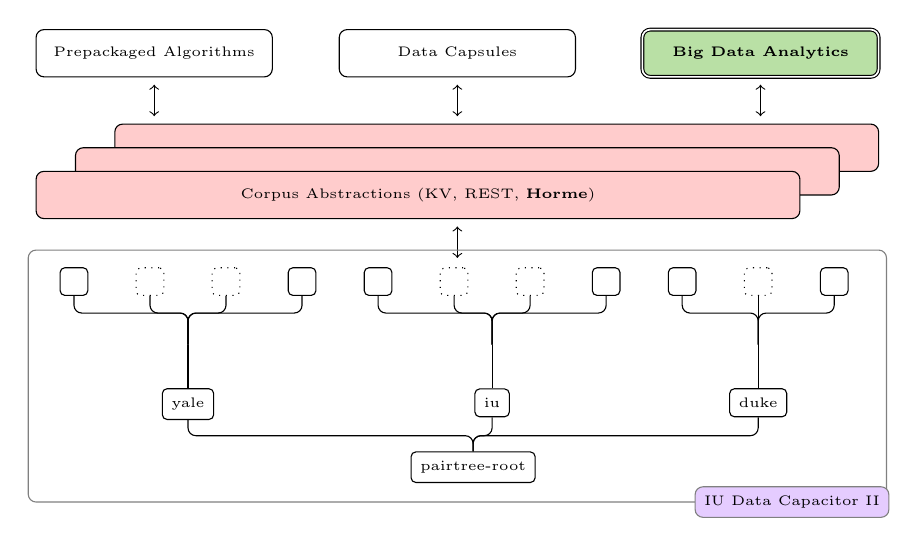
\begin{tikzpicture}
[   grow'=up,
    level distance=.8cm,
    sibling distance=.6cm,
    edge from parent fork up,
    edge from parent/.style={draw,rounded corners=1mm}
]
\begin{scope}[local bounding box=scope1]
  \draw[rounded corners=1mm] (-6.7,4.8) rectangle (-3.7,4.2) node[pos=.5] {\tiny Prepackaged Algorithms};
  \draw[rounded corners=1mm] (-2.85,4.8) rectangle (0.15,4.2) node[pos=0.5] {\tiny Data Capsules};
  \draw[rounded corners=1mm,fill=computegreen,double] (1,4.8) rectangle (4,4.2) node[pos=0.5] {\tiny \textbf{Big Data Analytics}};
  \draw[fill=datared,rounded corners=1mm] (-5.7,3.6) rectangle (4,3) ;
  \draw[fill=datared,rounded corners=1mm] (-6.2,3.3) rectangle (3.5,2.7) ;
  \draw[fill=datared,rounded corners=1mm] (-6.7,3) rectangle (3,2.4) node[pos=.5] {\tiny Corpus Abstractions (KV, REST, \textbf{Horme})};
\end{scope}
\draw[<->] (-1.35,2.3) -- (-1.35,1.9); %node[draw=orange,anchor=west,pos=0.5,circle,fill=red!20,inner sep=0pt,minimum size=10pt,xshift=2pt]{\footnotesize \textbf{1}};
\draw[<->] (-5.2,4.1) -- (-5.2,3.7); %node[draw=orange,anchor=west,pos=0.5,circle,fill=red!20,inner sep=0pt,minimum size=10pt,xshift=2pt]{\footnotesize \textbf{2}};
\draw[<->] (-1.35,4.1) -- (-1.35,3.7); %node[draw=orange,anchor=west,pos=0.5,circle,fill=red!20,inner sep=0pt,minimum size=10pt,xshift=2pt]{\footnotesize \textbf{3}};
\draw[<->] (2.5,4.1) -- (2.5,3.7); %node[draw=orange,anchor=west,pos=0.5,circle,fill=red!20,inner sep=0pt,minimum size=10pt,xshift=2pt]{\small \textbf{4}};
\begin{scope}[shift={($(scope1.north)+(0.2cm,-5.6cm)$)}]
  \tikzstyle{var} = [draw,shape=rectangle,minimum size=1em,rounded corners=0.6mm]
  \tikzstyle{operator} = [draw=none,fill=none,above,pos=0]
  \tikzset{every node/.style={var}}
  \Tree [.\tiny pairtree-root 
          [.\tiny yale [[.\node[] {}; ] [.\node[dotted] {}; ]  [.\node[dotted] {}; ] [.\node[] {}; ]]]
          [.\tiny iu [[.\node[] {}; ][.\node[dotted] {}; ] [.\node[dotted] {}; ][.\node[] {}; ]]]
          [.\tiny duke [[.\node[] {}; ] [.\node[dotted] {}; ] [.\node[] {}; ]] 
          ]
        ]
\end{scope}
\draw[rounded corners=1mm,draw,gray] (-6.8,2) rectangle (4.1,-1.2) node[fill=dcpurple,draw,pos=1,xshift=-1.2cm,rounded corners=1mm] {\tiny \textcolor{black}{IU Data Capacitor II}};
\end{tikzpicture}
\end{frame}

\begin{frame}[c]{Text Data Mining At HTRC}
  \begin{itemize}
    \item General pattern: 
    \begin{itemize}
      \item Reduce 14 million texts to 1 million to analyze
      \item Text storage is organized according to library  that owns digitzed book where access is  by genre, subject, etc.
    \end{itemize}
    \item HDFS performs poorly in random access use cases
    \item HBase good for random access, but needs to deploy external to HPC or HTC compute nodes due to transient nature of batch jobs
    \item HBase over Lustre is not optimal
  \end{itemize}
\end{frame}


\begin{frame}[c]{Hadoop on HPC and HTC Environments}
\begin{columns}[T] % align columns
\begin{column}{.48\textwidth}
\begin{figure}[t]
  \includegraphics[scale=0.5]{hadoop-on-hpc}
  \centering
\end{figure}
\end{column}%
\hfill%
\begin{column}{.48\textwidth}
General workflow:
\begin{enumerate}
  \item Setup Hadoop cluster
  \item Partition and stage in blocks of digitized texts
  \item Execute analysis algorithm
  \item Stage out analytical results
\end{enumerate}
\end{column}%
\end{columns}

\end{frame}

\begin{frame}[c]{Hadoop on HPC and HTC Environments}
  \begin{itemize}
    \item Data is stored in \emph{parallel file system, e.g., Lustre} connected to compute nodes via network
    \item Often data gets staged to scratch space in compute nodes (e.g. HDFS data nodes) from Lustre before actual computation
    \item Results get copied back to Lustre after job completion
    \item \textbf{High data staging overhead}
    \item HDFS on HPC and HTC environments limited by scratch space capacity of compute nodes
  \end{itemize}
\end{frame}

\section{Horme}

\begin{frame}[c]{Horme}
\begin{itemize}
  \item Indexed binary file format for packing key/value pairs where size of value range from couple of kilobytes to couple of megabytes
  \item Set of tools for packing and managing key/value pairs  
  \item Library for reading and writing indexed binary files 
  \item Storage extensions for popular Big Data processing frameworks to read and write Horme binary files
  \item Not tied to any processing framework
  \item Works on top of any file system
  \item Delegates replication, file striping and fault-tolerance to underlying file system
\end{itemize}
\end{frame}

\begin{frame}[c]{Horme - BloomHashIndexFile}
\begin{figure}[t]
  \includegraphics[scale=0.6]{horme-2}
  \centering
\end{figure}  
\end{frame}

\begin{frame}[c]{Horme - Programming Abstraction}
  \begin{itemize}
    \item Reader
    \begin{center}
      \begin{tabular}{| l | l |}
       \hline
       \textbf{Scan} & \texttt{for(Record r : BloomHashIndexFile)} \\ 
       \hline
       \textbf{Random Access} & \texttt{Record get(Key key)} \\  
       \hline
       \textbf{Membership Test} & \texttt{boolean probablyHasKey(Key key)} \\   
       % Milinda, ``probably'' is very unscientific term.  Be ready to defend it in probability or other more precise terms.   You may want to replace ``probably'' with a more precise term  so as to avoid scrutiny.  I looked at paper and it's not evident how the method is implemented. Surprised the reviewers (or me) didn't catch earlier. 
       \hline
       \textbf{Accessors} & \specialcell{\texttt{HashIndex getHashIndex()} \\ 
\texttt{BloomFilter getBloomFilter()}} \\    
       \hline
      \end{tabular}
    \end{center}
    \item Writer
    \begin{center}
      \begin{tabular}{| l | l |}
       \hline
       \textbf{Write} & \texttt{void append(Key key, Value val)} \\ 
       \hline
       \textbf{Misc.} & \texttt{int getLength()} \\  
       \hline
      \end{tabular}
    \end{center}
  \end{itemize}
\end{frame}

\begin{frame}[c]{Horme - Distributed Packing Utility}
  \begin{itemize}
    \item Pack key-value raw data into binary chunks
    \item Pleasingly parallel packing process
    \item For sake of load balancing each chunk should carry roughly same payload
    \begin{itemize}
      \item Same \# of records (e.g., simulation analysis task)
      \item Same chunk file size (e.g., text mining task)
    \end{itemize}
  \end{itemize}
\end{frame}

\begin{frame}[c]{Horme - Parallel Processing Layer}
  \begin{itemize}
    \item Hadoop input and output format extensions on top of BloomHashIndexFile
    \item Retains MapReduce key-value semantics 
    \item Supports both scan and random access 
    \item Binary chunks can be served from parallel file system or HDFS cluster coupled with Hadoop deployment
  \end{itemize}
\end{frame}

\begin{frame}[c]{Horme - Processing from Network Storage}
\begin{figure}[t]
  \includegraphics[scale=0.4]{horme-with-pfs}
  \centering
\end{figure}
\end{frame}

\begin{frame}[c]{Horme - Processing from Network Storage}
\begin{itemize}
  \item With NLineInputFormat, a single input split consists of N consecutive lines
  \item \texttt{BloomHashIndexFile} \texttt{Reader} reads value corresponding to each key in input split at mapper
  \item Input sorted by binary chunk path so that \texttt{RecordReader} need only open a new file when next line is a new chunk
  \item Workload balanced on number of records processed
  \item Workload approximately balanced on size of records 
\end{itemize}
\end{frame}

\begin{frame}[c]{Horme - Processing from HDFS}
  Horme Hadoop extensions determine input splits and convert input splits to key-value pairs for consumption by mappers
  \begin{figure}[t]
  \includegraphics[scale=0.3]{horme-hdfs}
  \centering
\end{figure}
\end{frame}

\section{Experimental Evaluation}

\begin{frame}[c]{Experimental Evaluation Environment}

\begin{itemize}
  \item Single node setting: 4-core 2.4 GHz Intel W3503 Xeon CPU, 8 GB RAM, 7200 RPM SATA drive 
  \item Distributed node setting: each node is two Intel Xeon E5-2650 v2 8-core processors, 32 GB RAM, 180 GB local disk at 7200 RPM 
  \item Each record has fixed sized key (100 byte) and value (2 MB)
  \item Hadoop v2.6.1
  \item 128 MB HDFS blocks with default replication factor of 3
  \item Lustre parallel file system
  \item Dataset size: 425,276 texts (digitized books)
\end{itemize}
\end{frame}

\begin{frame}[c]{Overhead of BloomHashIndexFile}
\vspace{-1.5cm}
\begin{columns}[T] % align columns
    \begin{column}{.48\textwidth}
    \begin{figure}[ht!]
      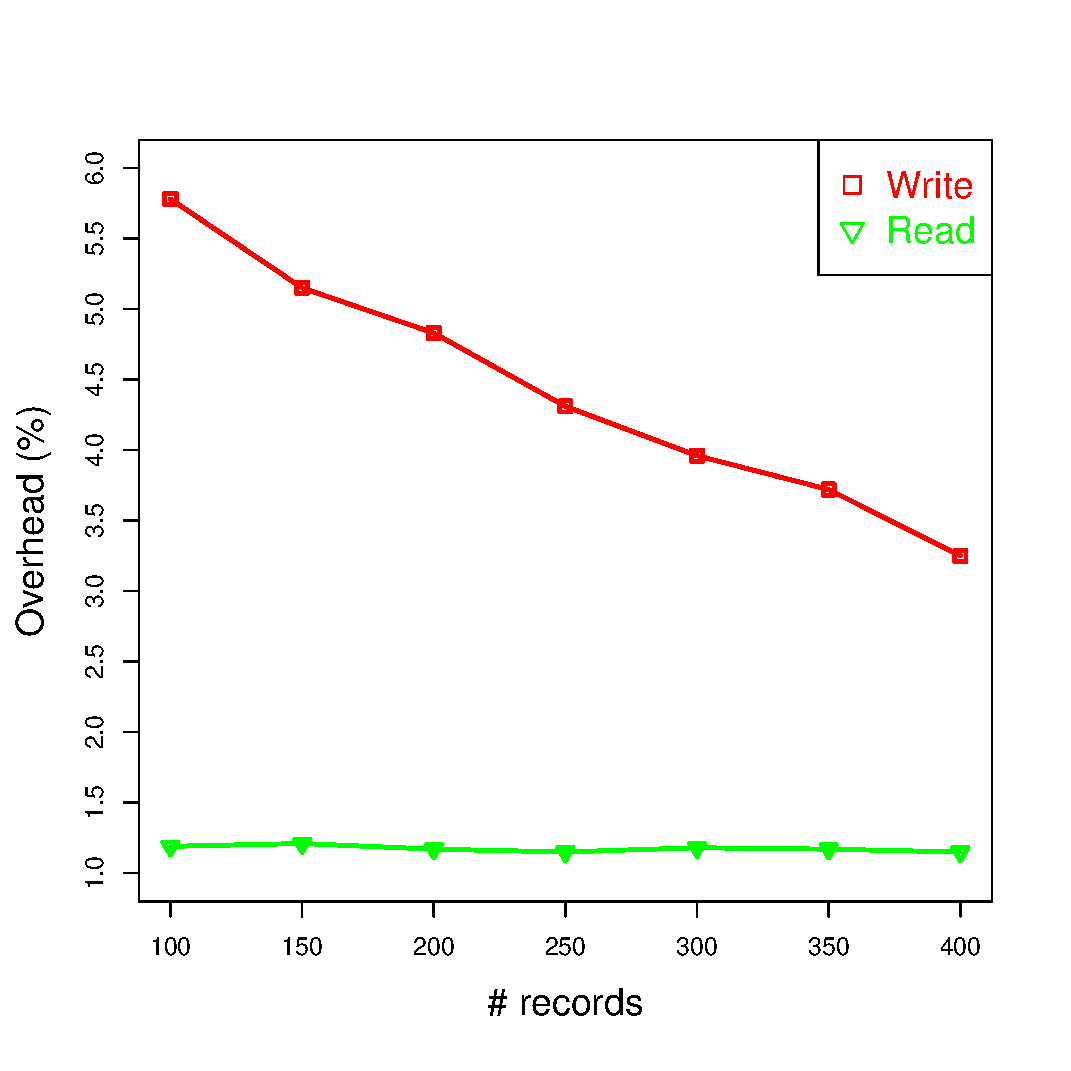
\includegraphics[scale=0.3]{exp-bloomhash-rw-overhead}
      \centering
    \end{figure}
    \end{column}%
    \hfill%
    \begin{column}{.48\textwidth}
    \begin{figure}[ht!]
      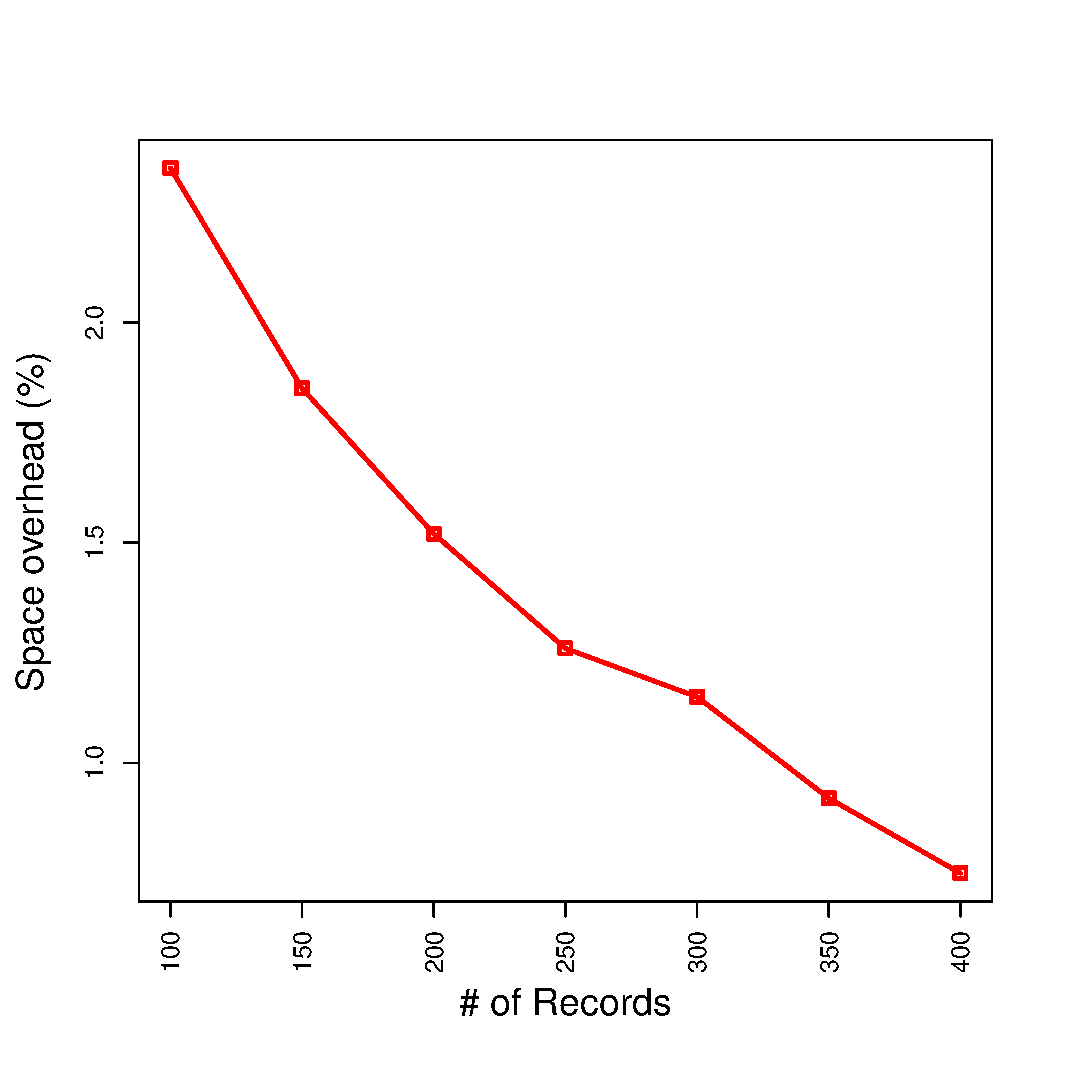
\includegraphics[scale=0.3]{exp-bloomhash-space-overhead}
      \centering
    \end{figure} 
    \end{column}%
\end{columns}  
\end{frame}

\begin{frame}[c]{Horme vs Vanilla Hadoop}
\vspace{-1.5cm}
\begin{columns}[T] % align columns
    \begin{column}{.48\textwidth}
    \begin{figure}[ht!]
      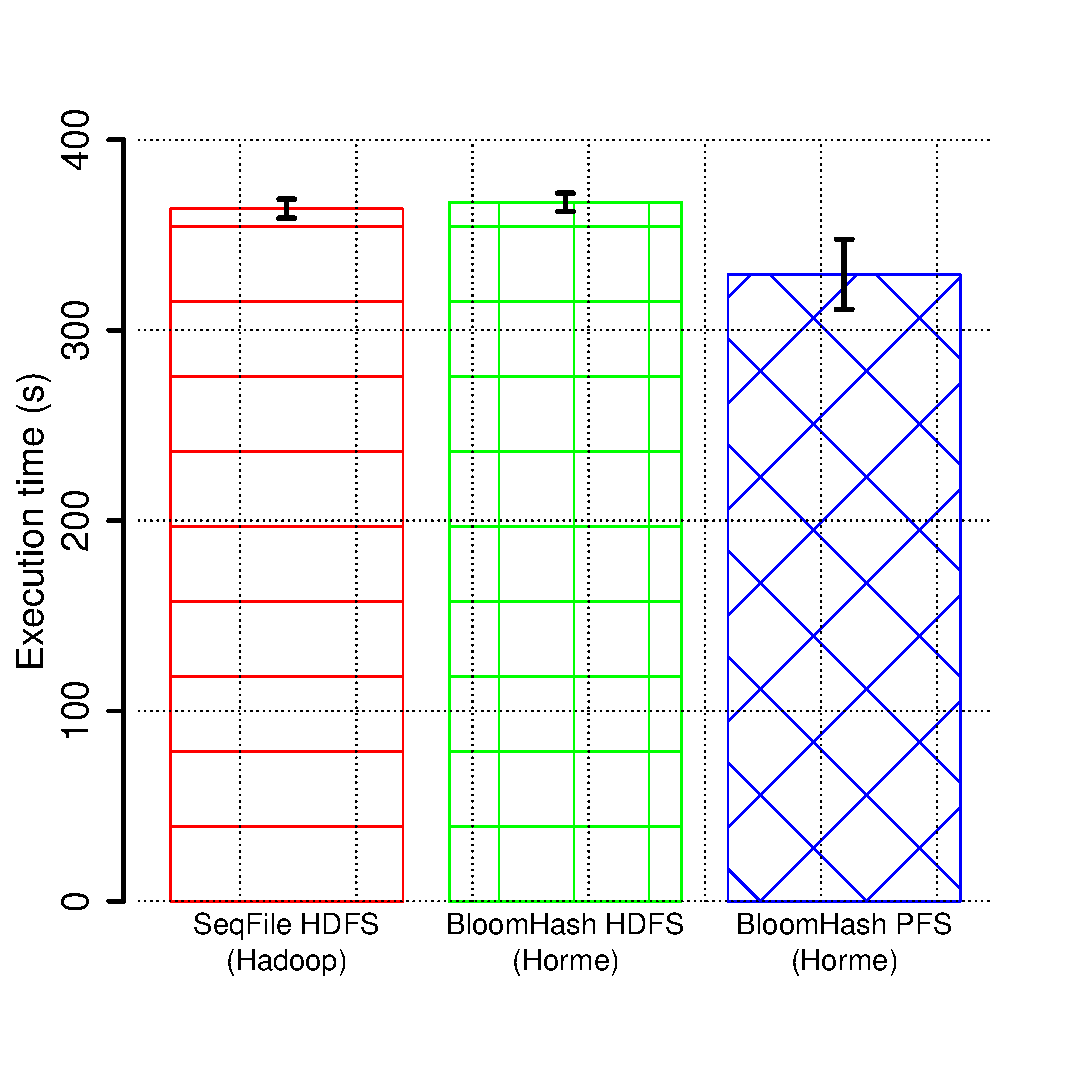
\includegraphics[scale=0.3]{eval-scan}
      \centering
      \caption{Scan/Sequential Access}
    \end{figure}
    \end{column}%
    \hfill%
    \begin{column}{.48\textwidth}
    \begin{figure}[ht!]
      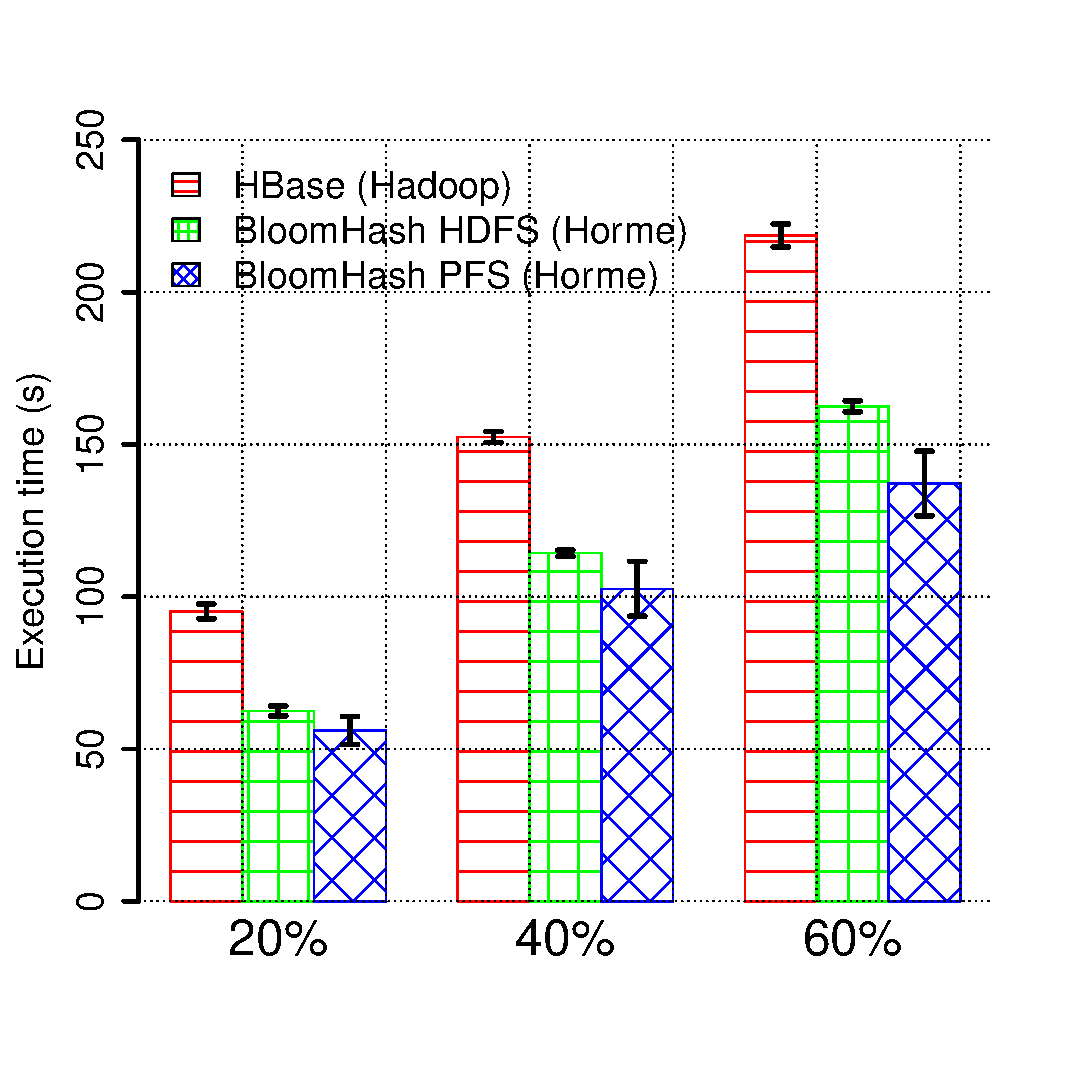
\includegraphics[scale=0.3]{eval-random}
      \centering
      \caption{Query/Random Access}
    \end{figure} 
    \end{column}%
\end{columns}  
\end{frame}

\begin{frame}[c]{Horme vs Vanilla Hadoop}
\begin{figure}[ht!]
      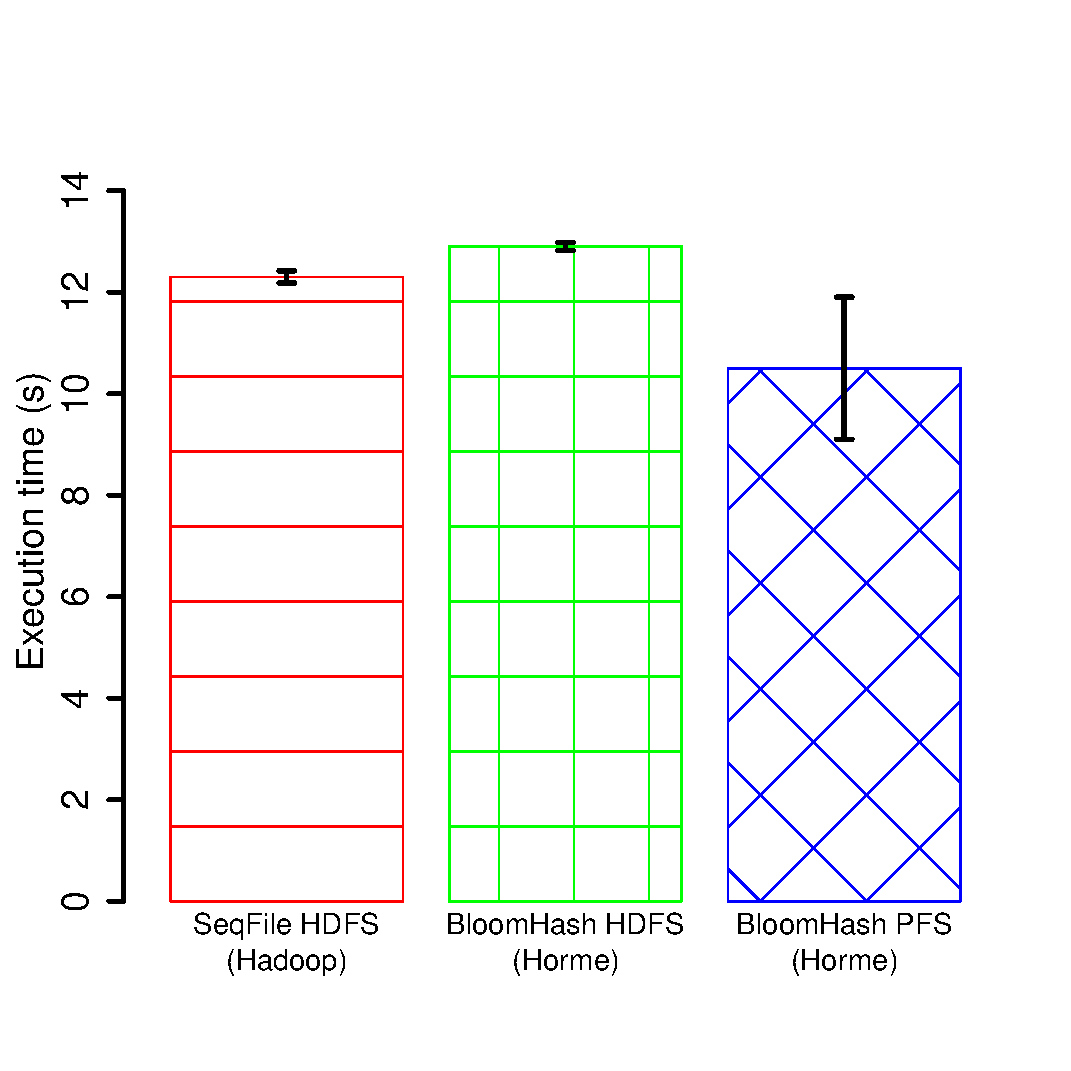
\includegraphics[scale=0.3]{eval-write}
      \centering
      \caption{Write}
    \end{figure}  
\end{frame}

\begin{frame}[c]{Observations}
  \begin{itemize}
    \item Horme’s “Random read from PFS” outperforms Hadoop’s “Random read from HBase” by 41.1\%, 32.7\%, and 37.3\% for 20\%, 40\% and 60\% query setting, respectively. 
    \item Horme superior to “Random read from HDFS” by 10.8\%, 10.2\% and 15.6\% respectively in three settings
  \end{itemize}
\end{frame}


\begin{frame}[c]{Related Work}
% Milinda, cite the 2-3 most closely related works here. You won't want to dwell on them in the talk, but will need to include this slide. 
  \begin{itemize}
    \item \small Fadika, Zacharia, et al. \textbf{"Mariane: Mapreduce implementation adapted for hpc environments."} 2011 IEEE/ACM 12th International Conference on Grid Computing. IEEE, 2011.
    \item \small Sehrish, Saba, et al. \textbf{"Mrap: A novel mapreduce-based framework to support hpc analytics applications with access patterns."} Proceedings of the 19th ACM International Symposium on High Performance Distributed Computing. ACM, 2010.
    \item \small Dong, Bo, et al. \textbf{"A novel approach to improving the efficiency of storing and accessing small files on hadoop: a case study by powerpoint files."} Services Computing (SCC), 2010 IEEE International Conference on. IEEE, 2010.
  \end{itemize}
\end{frame}

\begin{frame}[c]{Future Work}

  \begin{itemize}
    \item Improve read performance through delayed record fetching when reading BloomHashIndexFile
    \item Evaluation is over 500,000 texts (books); future work is to evaluate in realistic setting of HTRC 
    \item Horme's use in HTRC is for large-scale parallel pattern matching of n-gram (multi-word) terms on a large subset of HT corpus.  
    \item Open question around packing strategy that reduces random access time for 80\% of anticipated workload
  \end{itemize}
\end{frame}
\end{document}